To provide a good service, it's needed that TCP flows respond to orders given
by the hosts machines that controls the connection during congestion. This
characteristic of flows is called ``\textit{responsiveness}'' and tells when 
flows must back-off during congestion. In the second half of the 80's, TCP
began to experience a strange phenomenon that manifested itself through a
dramatically diminish throughput. After a deep analysis, Van Jacobson showed
that TCP needed a mechanism to limit transmission speed in the face of
congestion\cite{JacobsonCAC}. This lead to the development of a better
congestion control mechanism for TCP, which was added as a requirement for
hosts connected to Internet\cite{RFC1122}. Since then, the congestion controls
methods implemented in TCP has been updated several times, adding two new
algorithms, the \textit{slow start} and \textit{congestion avoidance} were
designed to keep in ``equilibrium'' the data that is in exchange. Later a
third where added, the \textit{fast retransmit and fast recovery}.

\subsubsection{Slow start and Congestion avoidance}

 \begin{wrapfigure}{r}{0.5\textwidth}
  \begin{center}
    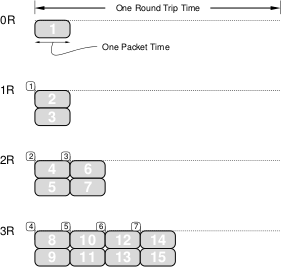
\includegraphics[width=0.48\textwidth]{img/slowstart}
  \end{center}
  \caption[The Chronology of a Slow-Start.]{The Chronology of a Slow-Start.\cite{JacobsonCAC}}
  \label{fig:slowstart}
\end{wrapfigure}

The idea behind bandwidth occupancy in TCP is to use as much as it is allow to
use. With this in mind, slow start proves the network by increasing
exponentially the rate of how many packets sends; the \gls{cwin} is
increases by one packet and adds another for each packet acknowledged. This
behavior continues until the \gls{ssthrsh} is reached or
congestion is signaled. If congestion is detected, the slow start threshold is
reset to half of the amount of congestion window, at the time that congestion
window is reset to a size of one segment, and slow start is restarted. In case
that the slow start threshold is reached, the sender switches to congestion
avoidance mode, which is employed to maintain the transmission rate,
increasing by one segment each RTT\footnote{Each ack increases the congestion
window by $ss*ss/cwnd$. This results in a linear increase of the congestion
window; that means in 1 RTT, congestion window will be increased by
1 \cite{JacobsonCAC} \cite{rfc879} \cite{rfc2460}}.

TCP must be smart enough to signal to the hosts when path is experiencing
congestion, so it must have policies that decrease the network utilization or
increase it if congestion signals are received or not. Also, based on the
afore mentioned principle (``\textit{packet conservation principle}''),
congestion collapse would become the exception rather than a rule. Thus
congestion control involves finding place that violate conservation and fixing
them. It is important detect early this misbehavior, since new packets are
added exponentially also the congestion grows exponentially, so if is detected
early, only small adjustments will cure it.

Typically, when the sender is signaled that packets are been dropped, TCP/IP
networks understand that as congestion, but typical effects include queuing
delay, packet loss or the blocking of new connections. New implementations
define a explicit congestion notification methods \cite{rfc3168}, that allows
notification of congestion between the ends without any packet loss. TCP
specification mandates initially setting the congestion window to between 2
and 4 segments of data depending on the segment size\cite{rfc3390}.

\subsubsection{Congestion control algorithms}
One of the biggest problems that TCP had in the past years for its development
has been the achieve of optimal utilization preventing congestion associated
with the differences of bandwidth existing in the medium through which
communication is propagated. That is why lately there have been various
implementations for proper handling of the original algorithm originally
deployed in TCP for attaining prevent or lessen the effects of this problem.
Among the algorithms that currently exist, the two predominant in modern
operating systems will be mentioned: CUBIC and Compound TCP.

\paragraph{CUBIC TCP}  is the default implementation for congestion control in
the Linux kernel since 2.6.19. \textit{Scaling the window growth rate to match
large \gls{BDP} is rather straightforward, tackling the fairness issues of new
protocols has remained as a major challenge.  Although BDP implies the network
capacity by packet count(or window size), packet count is not adequate to
characterize TCP performance because growth rate of TCP depends on
RTT}\cite{HaCubic}.

Because the basis of their growth is a cubic function (hence its name), has a
less aggressive behavior than their predecessors, while retaining excellent
scalability, fairness and stability. As can be seen in Figure
\ref{fig:cubicfunc}, the cubic function is compound of three parts: a concave
part where the window grows rapidly over small time values, a plateau set at the previous maximal
congestion window size, and the end portion where the increasing bandwidth
above the maximum which exhibits a convex shape.

As can be better seen in the formula at Figure \ref{fig:cubicform}, the congestion
window ain't dependent of its previous acknowledged packets; instead, the
congestion window is computed at each step from a calibrated function. With
this calibration, the plateau is at the previous maximal congestion window
size. This feature allow the algorithm to respond faster to changes in
available bandwidth. Since in previous algorithms throughput is defined by the
packet loss rate as well as RTT, the throughput in CUBIC is defined by only
the packet loss rate.

\begin{wrapfigure}{r}{0.5\textwidth}
    %\rule{5.5cm}{7.1cm}
\begin{center}
    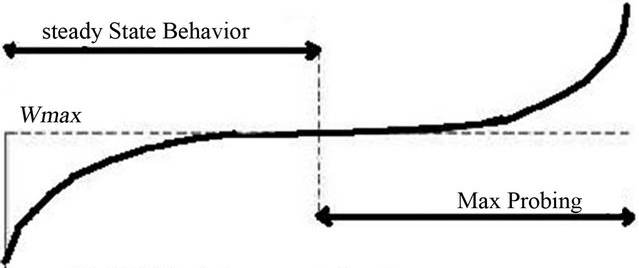
\includegraphics[width=0.48\textwidth]{img/cubic}
  \end{center}
\caption{The window growth function of CUBIC}
\label{fig:cubicfunc}
\end{wrapfigure}

Another feature that CUBIC has with respect to its predecessor in the Linux
kernel, it also changes the behavior of the Slow Start algorithm, replacing it
with

\begin{figure}[ht]
\begin{minipage}{6cm}
\centering
	\[ W_{cubic} = C(t - K)^3 + W_{max}\]
    \caption{CUBIC's Congestion Window.\protect\footnotemark}
    \label{fig:cubicform}
\end{minipage}%
\end{figure}%

\footnotetext{C is a scaling factor, textit{t} is the elapsed time from the
last window reduction. $W_{max}$ is the window size before the last window
reduction. $K=sqrt[3]{W_{max}beta/C}$. And $beta$ is a constant
multiplication decrease factor applied for window reduction at the time of
loss event}

\noindent  one called Hybrid Slow Start (or HyStart)\cite{HaElephants}. 
The idea behind this algorithm is to prevent the extra drop of packets caused by the
overshoot of bandwidth done by the regular slow start. This extra amount of
data cause unnecessary delay on both ends hosts and network, and taking long time to
recover from, that can be worst if the packet drop is made at a late stage of
the slow start\footnote{since slow start adds one extra packet for each
acknowledged}.

\paragraph{Compound TCP} is the modification to TCP stack algorithm promoted
for Microsoft and implemented in their systems since Windows Vista and Server
2008. This algorithm aims to achieve a significant improvement in resource
utilization by TCP, presenting an fair mix between delay-based approach and
loss-based approach.

CTCP is based in the idea that if the link is under-utilized, the protocol
should incraese the sending rate in a agressibly manner so it can obtain
available bandwidth more quickly. But when the link is nearly full
utilization, keep that aggressiveness is unproductive because at this stage it
is expected that the protocol is more accurate in achieving complete the
remaining bandwidth. So CTCP incorporates a scalable delay-based component
into the standard TCP congestion avoidance algorithm\cite{4146841}.

\begin{wrapfigure}{r}{0.5\textwidth}
    %\rule{5.5cm}{7.1cm}
  \begin{center}
    \[ win = min(cwnd + dwnd, awnd)\]
  \end{center}
  \caption{Compound TCP sending window.\protect\footnotemark}
  \label{fig:ctcpform}
\end{wrapfigure}

As can be seen in figure \ref{fig:ctcpform}, the congestion window or cwnd
which manages the loss-based component is untouched, and a delay window - dwnd
- is added to manage the delay-based component.  The awnd is the advertised
window from the receiver. This algorithm has shown that in periods of under-
utilization, it has an aggressive and scalable increase rule, and gradually it
reduce the sending rate accordingly when the network is sensed to be fully
utilized. But thanks to the packet loss component, it also reacts to packet
loss reducing the sending rate to keep the conservative property of TCP. Also,
Tan et al\cite{Tan06compoundtcp} has reveal that CTCP has a good performance
over current high BDP networks too.

\subsubsection{Fast retransmit and fast recovery} 
Timers are an important part of this self-regulated protocol. TCP maintains
four timers\footnote{The timers that TCP has for each connection are:
(1)Persist Timer: Ensures that window size information is transmitted even  if
no data is transmitted. (2)Keepalive Timer: Detects crashes on the other end
of the connection. (3)2MSL Timer: Measures the time that a connection has been
in the TIME\_WAIT state. (4)Retransmission Timer: The timer is started during
a transmission. A timeout causes a retransmission}. One of them, the
retransmission timer, causes the sender to retransmit the segment over which
at the expiry of this timer(which is a function of the estimated RTT), has not
yet received their respective acknowledge, assuming the segment is lost in the
network. When this action is unleashed, the server will interpret it as a sign
of congestion, but data still flowing.

As already seen in \textbf{2.2.2.1}, slow start can do a lot of damage to our
networks, but fast retransmit helps to recover from lost without hurting the
network that much. It is triggered after a specified number of
acknowledgments, usually is at the third, with the same acknowledge number are
received by the sender. This makes the sender reasonably confident that
the next higher sequence number was dropped and needs to be retransmitted; all
this without the need for the action triggered by the timeout.

Fast recovery manages the continuous transmitting of new data on subsequent
duplicate acknowledgments, until the retransmitted packet is received. and
after a non-duplicated acknowledge is received, the congestion window is reset
back to the value it had before the fast retransmit was initiated, and the
fast recovery mode is ended, going back to congestion avoidance mode.
